\chapter{Floating Point Numbers}
\label{chapter:floatingpoint}

\section{IEEE-754 Floating Point Number Representation}
\label{chapter::floatingpoint}

This section provides an overview of the IEEE-754 32-bit binary floating
point format.\cite{ieee:754}

\begin{itemize}
\item Recall that the place values for integer binary numbers are:
\begin{verbatim}
   ... 128 64 32 16 8 4 2 1
\end{verbatim}
\item We can extend this to the right in binary similar to the way we do for
decimal numbers:
\begin{verbatim}
   ... 128 64 32 16 8 4 2 1 . 1/2 1/4 1/8 1/16 1/32 1/64 1/128 ...
\end{verbatim}
The `.' in a binary number is a binary point, not a decimal point.

\item We use scientific notation as in $2.7 \times 10^{-47}$ to express either
small fractions or large numbers when we are not concerned every last digit
needed to represent the entire, exact, value of a number.

\item The format of a number in scientific notation is $mantissa \times base^{exponent}$

\item In binary we have $mantissa \times 2^{exponent}$

\item IEEE-754 format requires binary numbers to be {\em normalized} to
$1.significand \times 2^{exponent}$ where the {\em significand}
is the portion of the {\em mantissa} that is to the right of the binary-point.

\begin{itemize}
\item The unnormalized binary value of $-2.625$ is $-10.101$
\item The normalized value of $-2.625$ is $-1.0101 \times 2^1$
\end{itemize}

\item We need not store the `1.' part because {\em all} normalized floating
point numbers will start that way.  Thus we can save memory when storing
normalized values by inserting a `1.' to the left of significand.

\begin{figure}[H]
   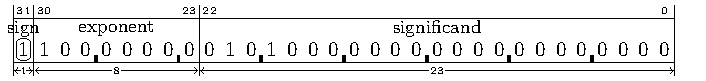
\includegraphics{figures/appendix02/floatNumber.pdf}
\end{figure}

%{
%\small
%\setlength{\unitlength}{.15in}
%\begin{picture}(32,4)(0,0)
%	\put(0,1){\line(1,0){32}}		% bottom line
%	\put(0,2){\line(1,0){32}}		% top line
%
%	\put(0,1){\line(0,1){2}}		% left vertical
%	\put(0,2){\makebox(1,1){\tiny 31}}	% left end bit number marker
%
%	\put(32,1){\line(0,1){2}}		% vertical right end
%	\put(31,2){\makebox(1,1){\tiny 0}}	% right end bit number marker
%
%	\put(0,0){\makebox(1,1){\small sign}}
%	\put(1,0){\makebox(8,1){\small exponent}}
%	\put(9,0){\makebox(23,1){\small significand}}
%
%    \put(0,1){\makebox(1,1){1}}		% sign
%
%	\put(1,1){\line(0,1){2}}		% seperator
%	\put(1,2){\makebox(1,1){\tiny 30}}	% bit marker
%
%    \put(1,1){\makebox(1,1){1}}		% exponent
%    \put(2,1){\makebox(1,1){0}}
%    \put(3,1){\makebox(1,1){0}}
%    \put(4,1){\makebox(1,1){0}}
%    \put(5,1){\makebox(1,1){0}}
%    \put(6,1){\makebox(1,1){0}}
%    \put(7,1){\makebox(1,1){0}}
%    \put(8,1){\makebox(1,1){0}}
%
%	\put(8,2){\makebox(1,1){\tiny 23}}	% bit marker
%	\put(9,1){\line(0,1){2}}		% seperator
%	\put(9,2){\makebox(1,1){\tiny 22}}	% bit marker
%
%    \put(9,1){\makebox(1,1){0}}
%    \put(10,1){\makebox(1,1){1}}
%    \put(11,1){\makebox(1,1){0}}
%    \put(12,1){\makebox(1,1){1}}
%    \put(13,1){\makebox(1,1){0}}
%    \put(14,1){\makebox(1,1){0}}
%    \put(15,1){\makebox(1,1){0}}
%    \put(16,1){\makebox(1,1){0}}
%    \put(17,1){\makebox(1,1){0}}
%    \put(18,1){\makebox(1,1){0}}
%    \put(19,1){\makebox(1,1){0}}
%    \put(20,1){\makebox(1,1){0}}
%    \put(21,1){\makebox(1,1){0}}
%    \put(22,1){\makebox(1,1){0}}
%    \put(23,1){\makebox(1,1){0}}
%    \put(24,1){\makebox(1,1){0}}
%    \put(25,1){\makebox(1,1){0}}
%    \put(26,1){\makebox(1,1){0}}
%    \put(27,1){\makebox(1,1){0}}
%    \put(28,1){\makebox(1,1){0}}
%    \put(29,1){\makebox(1,1){0}}
%    \put(30,1){\makebox(1,1){0}}
%    \put(31,1){\makebox(1,1){0}}
%\end{picture}
%}

%\item $-((1 + \frac{1}{4} + \frac{1}{16}) \times 2^{128-127}) = -(1 \frac{5}{16} \times 2^{1}) = -(1.3125 \times 2^{1}) = -2.625$
\item $-((1 + \frac{1}{4} + \frac{1}{16}) \times 2^{128-127}) = -((1 + \frac{1}{4} + \frac{1}{16}) \times 2^1) = -(2 + \frac{1}{2} + \frac{1}{8}) = -(2 + .5 + .125) = -2.625$

\item IEEE-754 formats:

\begin{tabular}{|l|l|l|}
\hline
				& IEEE-754 32-bit	& IEEE-754 64-bit	\\
\hline
sign			& 1 bit				& 1 bit			\\
exponent		& 8 bits (excess-127)			& 11 bits (excess-1023)		\\
mantissa		& 23 bits			& 52 bits		\\
max exponent	& 127				& 1023			\\
min exponent	& -126				& -1022			\\
\hline
\end{tabular}

\item When the exponent is all ones, the significand is all zeros, and
the sign is zero, the number represents positive infinity.

\item When the exponent is all ones, the significand is all zeros, and
the sign is one, the number represents negative infinity.

\item Observe that the binary representation of a pair of IEEE-754 numbers
(when one or both are positive) can be compared for magnitude
by treating them as if they are two's complement signed integers.
This is because an IEEE number is stored in {\em signed magnitude} format and
therefore positive floating point values will grow upward and downward in the
same fashion as for unsigned integers and that since negative floating point
values will have its MSB set, they will `appear` to be less than a positive
floating point value.

When comparing two negative IEEE float values by treating them both as two's
complement signed integers, the order will be reversed because IEEE float values
with larger (that is, increasingly negative) magnitudes will appear to decrease
in value when interpreted as signed integers.

This works this way because excess notation is used in the format of the
exponent and why the significand's sign bit is located on the left of
the exponent.\footnote{I know this is true and was done on purpose because
Bill Cody, chairman of IEEE committee P754 that designed the IEEE-754 standard,
told me so personally circa 1991.}

\item Note that zero is a special case number.  Recall that a normalized
number has an implied 1-bit to the left of the significand\ldots\ which
means that there is no way to represent zero!
Zero is represented by an exponent of all-zeros and a significand of
all-zeros.  This definition allows for a positive and a negative zero
if we observe that the sign can be either 1 or 0.

\item On the number-line, numbers between zero and the smallest fraction in
either direction are in the {\em \gls{underflow}} areas.
\ednote{Need to add the standard lecture number-line diagram showing
where the over/under-flow areas are and why.}

\item On the number line, numbers greater than the mantissa of all-ones and the
largest exponent allowed are in the {\em \gls{overflow}} areas.

\item Note that numbers have a higher resolution on the number line when the
exponent is smaller.

\item The largest and smallest possible exponent values are reserved to represent
things requiring special cases. For example, the infinities, values representing
``not a number'' (such as the result of dividing by zero), and for a way to represent
values that are not normalized. For more information on special cases see \cite{ieee:754}.

\end{itemize}

\subsection{Floating Point Number Accuracy}
Due to the finite number of bits used to store the value of a floating point
number, it is not possible to represent every one of the infinite values
on the real number line.  The following C programs illustrate this point.


\subsubsection{Powers Of Two}
Just like the integer numbers, the powers of two that have bits to represent
them can be represented perfectly\ldots\ as can their sums (provided that the
significand requires no more than 23 bits.)

\listing{examples/appendix02/powersoftwo.c}{Precise Powers of Two}
\listing{examples/appendix02/powersoftwo.out}{Output from {\tt powersoftwo.c}}

\subsubsection{Clean Decimal Numbers}
When dealing with decimal values, you will find that they don't map simply
into binary floating point values.
% (the same holds true for binary integer numbers).

Note how the decimal numbers are not accurately represented as they get larger.
The decimal number on line 10 of \listingRef{examples/appendix02/cleandecimal.out}
can be perfectly represented in IEEE format.  However, a problem arises in
the 11Th loop iteration.  It is due to the fact that the
binary number can not be represented accurately in IEEE format.  Its least
significant bits were truncated in a best-effort attempt at rounding the value
off in order to fit the value into the bits provided.  This is an example of
{\em low order truncation}.  Once this happens, the value of \verb@x.f@ is
no longer as precise as it could be given more bits in which to save its value.

\listing{examples/appendix02/cleandecimal.c}{Print Clean Decimal Numbers}
\listing{examples/appendix02/cleandecimal.out}{Output from {\tt cleandecimal.c}}


\subsubsection{Accumulation of Error}

These rounding errors can be exaggerated when the number we multiply
the \verb@x.f@ value by is, itself, something that can not be accurately
represented in IEEE
form.\footnote{Applications requiring accurate decimal values, such as
financial accounting systems, can use a packed-decimal numeric format
to avoid unexpected oddities caused by the use of binary numbers.}
\ednote{In a lecture one would show that one tenth is a repeating
non-terminating binary number that gets truncated.  This discussion
should be reproduced here in text form.}

For example, if we multiply our \verb@x.f@ value by $\frac{1}{10}$ each time,
we can never be accurate and we start accumulating errors immediately.

\listing{examples/appendix02/erroraccumulation.c}{Accumulation of Error}
\listing{examples/appendix02/erroraccumulation.out}{Output from {\tt erroraccumulation.c}}


\subsection{Reducing Error Accumulation}

In order to use floating point numbers in a program without causing
excessive rounding problems an algorithm can be redesigned such that the
accumulation is eliminated.
This example is similar to the previous one, but this time we recalculate the
desired value from a known-accurate integer value.
Some rounding errors remain present, but they can not accumulate.

\listing{examples/appendix02/errorcompensation.c}{Accumulation of Error}
\listing{examples/appendix02/errorcompensation.out}{Output from {\tt erroraccumulation.c}}